% !TEX program = pdflatex
% !TEX TS-program = pdflatex
% !TEX encoding = UTF-8 Unicode
\documentclass[letterpaper, 10 pt, conference]{ieeeconf}
\usepackage{graphicx}
\overrideIEEEmargins
\IEEEoverridecommandlockouts

\usepackage[utf8]{inputenc}
\usepackage[T1]{fontenc}
\usepackage{amsmath}
\usepackage{amssymb}
\usepackage{booktabs}
\usepackage{multirow}
\usepackage{microtype}
\usepackage{etoolbox}
\usepackage{url}

% Rótulos en español (ieeeconf.cls los fija en inglés)
\makeatletter
\def\fnum@table{TABLA~\thetable}
\patchcmd{\thebibliography}{\section*{References}}{\section*{Referencias}}{}{}
\patchcmd{\thebibliography}{{References}}{{Referencias}}{}{}
\makeatother

\setlength{\textfloatsep}{2pt plus 1pt minus 1pt}
\setlength{\floatsep}{2pt plus 1pt minus 1pt}
\setlength{\intextsep}{2pt plus 1pt minus 1pt}
\setlength{\abovecaptionskip}{1.2pt}
\setlength{\belowcaptionskip}{0pt}
\setcounter{topnumber}{4}
\setcounter{bottomnumber}{4}
\setcounter{totalnumber}{6}
\renewcommand{\topfraction}{0.95}
\renewcommand{\bottomfraction}{0.95}
\renewcommand{\textfraction}{0.05}
\renewcommand{\floatpagefraction}{0.90}
\renewcommand{\baselinestretch}{0.92}
\IEEEaftertitletext{\vspace{-1.3\baselineskip}}
\makeatletter
\def\section{\@startsection{section}{1}{\z@}{0.60ex plus 0.15ex minus 0.1ex}{0.15ex plus 0.05ex minus 0ex}{\normalfont\normalsize\centering\scshape}}
\makeatother
\emergencystretch=1.5em

\title{\LARGE \bf
Clasificación de Sonidos Ambientales y de la Naturaleza mediante el Ajuste Fino del Audio Spectrogram Transformer
}

\author{Otto Wilmer Castillo Santacruz, Edgar Andrés Pérez Mora y Silvio Yopasa Romero\\
\textit{Maestría en Inteligencia Artificial (MAIA), Universidad de los Andes, Bogotá, Colombia}\\
{\tt\small \{o.castillos, ea.perezm1, s.yopasa\}@uniandes.edu.co}
}

\begin{document}

\maketitle
\thispagestyle{empty}
\pagestyle{empty}

%%%%%%%%%%%%%%%%%%%%%%%%%%%%%%%%%%%%%%%%%%%%%%%%%%%%%%%%%%%%%%%%%%%%%%%%%%%%%%%%
\section{Introducción}

La clasificación automática de sonidos ambientales y naturales permite identificar fuentes como cantos de aves, lluvia, viento, mamíferos o maquinaria urbana \cite{c1}. Esta tarea es clave para el monitoreo bioacústico de ecosistemas, la detección temprana de perturbaciones (p.~ej., motosierras o incendios) y el etiquetado multimedia. Sin embargo, las grabaciones ambientales presentan envolventes aperiódicas, transientes breves y ruido de fondo variable, lo que limita a los descriptores acústicos agregados en el tiempo \cite{c1}.

Los modelos basados en \textit{Transformers} \cite{c2} superaron el procesamiento secuencial mediante la autoatención multicabeza, relacionando en paralelo dependencias de largo alcance. Tras su extensión a imágenes con el \textit{Vision Transformer} (ViT) \cite{c3}, el \textit{Audio Spectrogram Transformer} (AST) \cite{c4} adaptó esta arquitectura al dominio acústico convirtiendo la onda en espectrogramas log-Mel divididos en parches bidimensionales. Al partir de pesos preentrenados en AudioSet \cite{c5}, AST modela interacciones globales entre bandas de frecuencia e instantes temporales.

El objetivo es realizar el ajuste fino durante $2$ épocas y la evaluación integral de AST sobre las $50$ clases ($5$ macro-categorías) de ESC-50 \cite{c1}. El enfoque integra: (i) conversión reproducible a espectrogramas log-Mel de $512$ cuadros con recorte posicional exacto; (ii) contraste controlado en validación frente a un modelo clásico y AST congelado; (iii) reentrenamiento final por $2$ épocas; y (iv) evaluación cuantitativa y cualitativa en el \textit{fold} independiente ($n=400$), logrando $93.00\,\%$ de exactitud y $92.75 \pm 9.55\,\%$ de \textit{F1 macro}.

%%%%%%%%%%%%%%%%%%%%%%%%%%%%%%%%%%%%%%%%%%%%%%%%%%%%%%%%%%%%%%%%%%%%%%%%%%%%%%%%
\section{Metodología}

\textbf{Conjunto de datos y preprocesamiento.}
Se empleó ESC-50 \cite{c1} desde el espejo público indicado (\textit{fold}~1) \cite{c6}: $2\,000$ clips de $5.0\,\text{s}$ a $44.1\,\text{kHz}$ en $50$ clases balanceadas ($40$/clase) y $5$ macro-categorías (\textit{Animales}, \textit{Naturaleza y agua}, \textit{Humanos (no habla)}, \textit{Interiores y domésticos}, \textit{Exteriores y urbanos}; $400$/grupo). La auditoría confirmó cero nulos, cero clips mudos y cero duplicados MD5, con marcado contraste energético entre \textit{Exteriores y urbanos} ($-19.42\,\text{dBFS}$, $7.9\,\%$ de silencio) e \textit{Interiores y domésticos} ($-27.31\,\text{dBFS}$, $35.6\,\%$ de silencio).

Cada audio se promedió a mono, remuestreó a $16\,\text{kHz}$ \cite{c5} y transformó a espectrogramas log-Mel Kaldi de $128$ bandas (ventana $25\,\text{ms}$, paso $10\,\text{ms}$; $498$ cuadros útiles). Fijar longitud máxima de $512$ cuadros conserva el $100\,\%$ de la señal real con $2.73\,\%$ de relleno (vs.~$51.37\,\%$ en $1\,024$) y reduce $\sim 4\times$ el costo cuadrático de atención \cite{c2}. Para preservar contrastes energéticos, se aplicó la estandarización global de AudioSet $(X-\mu)/(2\sigma)$ ($\mu=-4.2677$, $\sigma=4.5690$), llevando los $498$ cuadros activos de entrenamiento de $-6.8208 \pm 5.3665$ a $-0.2794 \pm 0.5873$. En entrenamiento se evaluó \textit{SpecAugment} \cite{c7} (máscaras de hasta $24$ bandas y $64$ cuadros).

\textbf{Partición y protocolo experimental.}
El \textit{fold}~1 ($n=400$, $8$/clase) quedó aislado para una única evaluación cuantitativa final. Como el espejo \cite{c6} omite el identificador de \textit{fold} y archivo fuente en el bloque de entrenamiento ($1\,600$ clips), este se dividió estratificadamente ($75\,\%/25\,\%$, semilla $42$) en entrenamiento ($n=1\,200$) y validación ($n=400$), sin fuga entre particiones. En validación se compararon cinco configuraciones por $2$ épocas con $600$ clips de entrenamiento ($50\,\%$ estratificado); la ganadora en \textit{F1 macro} se reentrenó con el $100\,\%$ ($n=1\,200$) por $2$ épocas.

\textbf{Arquitectura, pérdida y optimización.}
Se adaptó el modelo preentrenado \texttt{MIT/ast-finetuned-}\allowbreak\texttt{audioset-10-10-0.4593} \cite{c4, c5}. Una convolución $2\text{D}$ ($16\times 16$, paso $10\times 10$) extrae $12\times 50 = 600$ parches de $768$ dimensiones. Para conservar los pesos posicionales de AudioSet, los \textit{embeddings} posicionales $2\text{D}$ se recortaron estructuralmente de $1\,214$ a $602$ tokens (\texttt{[CLS]}, \texttt{[DIST]} y $50$ pasos temporales). Tras $12$ capas ($12$ cabezales, $d_k=64$), el promedio $\mathbf{h}_{\text{pool}}=\frac{1}{2}(\mathbf{h}_{\text{CLS}}+\mathbf{h}_{\text{DIST}})\in\mathbb{R}^{768}$ pasa por normalización de capa y una proyección lineal a $50$ salidas ($85.76\,\text{M}$ parámetros totales; $40.0\,\text{k}$ en la cabeza).

Con activación \textit{softmax}, $\hat{p}_c(x) = e^{z_c}/\sum_{j=0}^{49} e^{z_j}$, se minimizó la entropía cruzada categórica:
\begin{equation}
\mathcal{L}(\mathbf{z}, y) = -\log \hat{p}_y(x) = -z_y + \log\sum_{j=0}^{49} e^{z_j}.
\label{eq:ce}
\end{equation}
Se contrastaron: (1) referencia clásica de $246$ rasgos ($40$ MFCC, primeras y segundas derivadas, RMS, cruces por cero y centroide espectral en media/DE, escalados solo en entrenamiento) con regresión logística multinomial; (2) AST congelado ($\eta=10^{-3}$); y ajuste fino con (3) $\eta=3\times 10^{-5}$, (4) $\eta=5\times 10^{-5}$ y (5) $\eta=5\times 10^{-5}$ + \textit{SpecAugment}. Se usó AdamW ($\lambda=0.01$, excluyendo sesgos y LayerNorm) \cite{c8}, calentamiento lineal del $10\,\%$, lotes de $8$ ($16$ en evaluación), recorte $\|\nabla\|_2 \le 1.0$ y precisión mixta de $16$ bits. Se reportan exactitud \textit{Top-1} y \textit{Top-3} (para detectar clases cercanas entre $50$ categorías), precisión y sensibilidad macro, y \textit{F1 macro} $\pm$ DE entre las $50$ clases.

%%%%%%%%%%%%%%%%%%%%%%%%%%%%%%%%%%%%%%%%%%%%%%%%%%%%%%%%%%%%%%%%%%%%%%%%%%%%%%%%
\section{Resultados}

\textbf{Comparación cuantitativa en validación.}
La Tabla~\ref{tab:comparacion_val} muestra el desempeño en validación ($n=400$). La referencia MFCC obtuvo $43.62\,\%$ de \textit{F1 macro} y AST congelado subió a $90.59\,\%$ gracias a AudioSet \cite{c5}. Descongelar las $12$ capas superó $92.8\,\%$ y redujo la dispersión entre clases. \textbf{AST + SpecAugment ($\eta = 5\times 10^{-5}$)} lideró con $94.80 \pm 7.52\,\%$ de \textit{F1 macro} ($95.00\,\%$ exactitud), aunque su ventaja de $+0.37\,\text{pp}$ sobre la variante sin aumento equivale a uno o dos clips con una semilla.

\begin{table}[!t]
\centering
\caption{Comparación en validación ($n=400$) tras $2$ épocas con $600$ clips de entrenamiento (semilla $42$). \textit{F1 $\pm$ DE} indica media y DE entre las $50$ clases.}
\label{tab:comparacion_val}
\renewcommand{\arraystretch}{0.95}
\setlength{\tabcolsep}{3.4pt}
\resizebox{8.6cm}{!}{
\begin{tabular}{lccccc}
\toprule
\textbf{Configuración} & \textbf{Parám.} & \textbf{Pérdida} & \textbf{Acc (\%)} & \textbf{Top-3 (\%)} & \textbf{F1 Macro $\pm$ DE (\%)} \\
\midrule
1. MFCC + Reg. Logística & $12.4\text{ k}$ & $2.3368$ & $44.50$ & $61.75$ & $43.62 \pm 21.23$ \\
2. AST congelado ($\eta=10^{-3}$)* & $40.0\text{ k}$ & $0.5199$ & $90.75$ & $98.25$ & $90.59 \pm 12.80$ \\
3. AST ajuste fino ($\eta=3\cdot 10^{-5}$) & $85.8\text{ M}$ & $0.4158$ & $93.00$ & $99.25$ & $92.82 \pm 8.88$ \\
4. AST ajuste fino ($\eta=5\cdot 10^{-5}$) & $85.8\text{ M}$ & $\mathbf{0.2546}$ & $94.50$ & $99.25$ & $94.43 \pm 8.50$ \\
5. \textbf{AST + SpecAugment ($\eta=5\cdot 10^{-5}$)} & $\mathbf{85.8\text{ M}}$ & $0.2632$ & $\mathbf{95.00}$ & $\mathbf{99.50}$ & $\mathbf{94.80 \pm 7.52}$ \\
\bottomrule
\multicolumn{6}{l}{\footnotesize *600 clips indexados sobre el caché de representaciones extraído en orden barajado.}
\end{tabular}}
\end{table}

\textbf{Convergencia y desempeño en prueba.}
Al reentrenar la variante ganadora con el $100\,\%$ de entrenamiento ($n=1\,200$), la pérdida de validación bajó de $0.6267$ (época $0.5$) a $0.1213$ (época $2.0$), logrando $96.98 \pm 5.72\,\%$ de \textit{F1 macro} ($97.00\,\%$ de exactitud; $100.00\,\%$ \textit{Top-3}, Fig.~\ref{fig:quant_eval}(b)), frente a $50.70 \pm 22.72\,\%$ del modelo MFCC en validación.

\begin{figure}[!t]
\centering
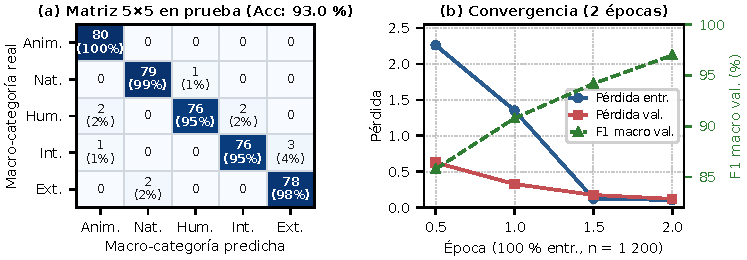
\includegraphics[width=0.98\linewidth]{figs/mp4_quant_eval.pdf}
\caption{Evaluación del AST final: (a) Matriz agregada $5\times 5$ en prueba ($n=400$; exactitud en $50$ clases: $93.00\,\%$); (b) Convergencia de pérdida y \textit{F1 macro} en validación durante $2$ épocas ($100\,\%$ de entrenamiento).}
\label{fig:quant_eval}
\end{figure}

\begin{table}[!t]
\centering
\caption{Desempeño en prueba (\textit{fold}~1, $n=400$) por macro-categoría ($80$ clips c/u) y global en $50$ clases.}
\label{tab:test_macro}
\renewcommand{\arraystretch}{0.95}
\setlength{\tabcolsep}{3.4pt}
\resizebox{8.6cm}{!}{
\begin{tabular}{lccccc}
\toprule
\textbf{Macro-categoría} & \textbf{Acc (\%)} & \textbf{Prec. (\%)} & \textbf{Sens. (\%)} & \textbf{F1 AST (\%)} & \textbf{F1 MFCC (\%)} \\
\midrule
Animales ($80$) & $\mathbf{100.00}$ & $\mathbf{97.27}$ & $\mathbf{100.00}$ & $\mathbf{98.42}$ & $45.80$ \\
Interiores y domésticos ($80$) & $91.25$ & $93.02$ & $91.25$ & $91.87$ & $42.78$ \\
Naturaleza y agua ($80$) & $92.50$ & $92.44$ & $92.50$ & $91.55$ & $44.66$ \\
Humanos (no habla) ($80$) & $90.00$ & $93.99$ & $90.00$ & $91.34$ & $48.63$ \\
Exteriores y urbanos ($80$) & $91.25$ & $91.19$ & $91.25$ & $90.59$ & $27.10$ \\
\midrule
\textbf{Global 50 clases ($n=400$)} & $\mathbf{93.00}$ & $\mathbf{93.58}$ & $\mathbf{93.00}$ & $\mathbf{92.75 \pm 9.55}$ & $41.79 \pm 23.07$ \\
\bottomrule
\end{tabular}}
\end{table}

En la prueba independiente (\textit{fold}~1, Tabla~\ref{tab:test_macro}), AST alcanzó \textbf{$93.00\,\%$ de exactitud} ($372/400$), \textbf{$98.75\,\%$ \textit{Top-3}}, \textbf{$92.75 \pm 9.55\,\%$ de \textit{F1 macro}} y pérdida de $0.2608$. Superó en $+50.96\,\text{pp}$ de \textit{F1 macro} al modelo MFCC ($42.25\,\%$ de exactitud; $41.79 \pm 23.07\,\%$ de F1; pérdida de $2.5674$). \textit{Animales} obtuvo $100\,\%$ de exactitud ($80/80$), y en la matriz $5\times 5$ (Fig.~\ref{fig:quant_eval}(a)) todos los bloques alcanzaron F1 $\geq 96.2\,\%$.

\begin{table}[!t]
\centering
\caption{Extremos por clase en prueba ($n=8$/clase): resumen de $22$ clases perfectas y las $6$ más retadoras.}
\label{tab:test_extremos}
\renewcommand{\arraystretch}{0.95}
\setlength{\tabcolsep}{3.0pt}
\resizebox{8.6cm}{!}{
\begin{tabular}{lcccc}
\toprule
\textbf{Categoría (Grupo)} & \textbf{TP/FN/FP} & \textbf{Prec. / Sens. (\%)} & \textbf{F1 AST (MFCC)} & \textbf{Confusión principal} \\
\midrule
22 clases perfectas* & $8/0/0$ & $100.0 / 100.0$ & $100.00$ ($25\text{–}78$) & Ninguna ($0$ errores) \\
\midrule
\texttt{washing\_machine} (Int.) & $4/4/2$ & $66.7 / 50.0$ & $57.14$ ($28.57$) & \texttt{engine} ($2$), \texttt{train} ($1$) \\
\texttt{wind} (Nat.) & $4/4/1$ & $80.0 / 50.0$ & $61.54$ ($0.00$) & \texttt{sea\_waves} ($4$) \\
\texttt{crying\_baby} (Hum.) & $5/3/0$ & $100.0 / 62.5$ & $76.92$ ($73.68$) & \texttt{cat} ($2$), \texttt{laughing} ($1$) \\
\texttt{footsteps} (Hum.) & $6/2/1$ & $85.7 / 75.0$ & $80.00$ ($9.09$) & \texttt{keyboard\_typ.} ($1$), \texttt{knock} ($1$) \\
\texttt{vacuum\_cleaner} (Int.) & $6/2/1$ & $85.7 / 75.0$ & $80.00$ ($15.38$) & \texttt{washing\_machine} ($2$) \\
\texttt{sea\_waves} (Nat.) & $8/0/4$ & $66.7 / 100.0$ & $80.00$ ($35.29$) & $4$ FP desde \texttt{wind} \\
\bottomrule
\multicolumn{5}{l}{\footnotesize *Empate de $22/50$ clases (p.~ej., \texttt{brushing\_teeth}, \texttt{chirping\_birds}, \texttt{clock\_tick}, \texttt{cow}, \texttt{dog}).}
\end{tabular}}
\end{table}

\textbf{Categorías extremas y patrones de error.}
La Tabla~\ref{tab:test_extremos} resume los extremos por clase. Un total de $22$ categorías ($44\,\%$) obtuvieron $100.00\,\%$ de F1, y las mayores caídas ocurrieron en \texttt{washing\_machine} ($57.14\,\%$) y \texttt{wind} ($61.54\,\%$). De los $28$ errores en prueba ($7.00\,\%$), $17$ ($60.7\,\%$) fueron intra-macro-grupo y $11$ ($39.3\,\%$) inter-grupo; cuatro pares concentraron $10$ errores: \texttt{wind} $\to$ \texttt{sea\_waves} ($4$), \texttt{crying\_baby} $\to$ \texttt{cat} ($2$), \texttt{vacuum\_cleaner} $\to$ \texttt{washing\_machine} ($2$) y \texttt{washing\_machine} $\to$ \texttt{engine} ($2$).

\textbf{Resultados cualitativos, espacio latente y robustez.}
En prueba, la mediana de probabilidad máxima separó los $372$ aciertos ($98.8\,\%$) de los $28$ errores ($73.1\,\%$). La Fig.~\ref{fig:qual_specs} contrasta espectrogramas reales de aciertos y errores, evidenciando similitud en impulsos y bandas estacionarias. La oclusión de parches en \texttt{pouring\_water} solo redujo $\Delta P \le 0.35\,\text{pp}$ por saturación \textit{softmax}.

En el espacio latente ($\mathbb{R}^{768}$), la proyección t-SNE \cite{c9} mostró grupos más compactos tras el ajuste fino: la silueta coseno de $50$ clases pasó de $0.3576$ a $0.5546$ ($\Delta=+0.1970$; euclidiana de $0.2188$ a $0.3682$). En los $5$ clips más confiables de prueba (\texttt{pouring\_water}, \texttt{door\_wood\_creaks}, \texttt{insects}, \texttt{chainsaw}, \texttt{brushing\_teeth}), AST acertó $20/20$ pruebas bajo señal limpia, ruido ($\text{SNR}=15\,\text{dB}$), atenuación ($-6\,\text{dB}$) y desplazamiento ($+1.5\,\text{s}$), con probabilidades entre $99.56\,\%$ y $99.85\,\%$.

\begin{figure}[!t]
\centering
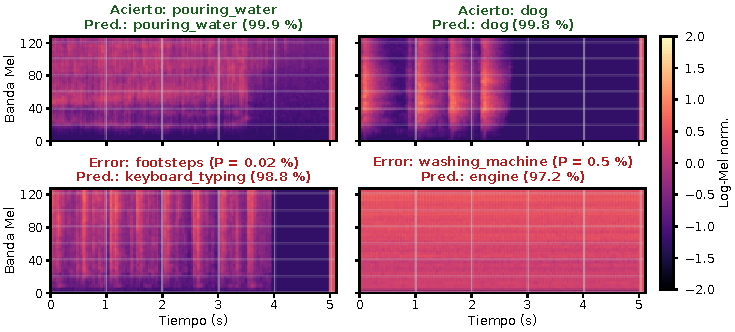
\includegraphics[width=0.98\linewidth]{figs/mp4_qual_eval.pdf}
\caption{Espectrogramas log-Mel normalizados reales de prueba: (arriba) aciertos en \texttt{pouring\_water} y \texttt{dog}; (abajo) errores de alta confianza en patrones impulsivos (\texttt{footsteps} $\to$ \texttt{keyboard\_typing}) y bandas estacionarias (\texttt{washing\_machine} $\to$ \texttt{engine}).}
\label{fig:qual_specs}
\end{figure}

%%%%%%%%%%%%%%%%%%%%%%%%%%%%%%%%%%%%%%%%%%%%%%%%%%%%%%%%%%%%%%%%%%%%%%%%%%%%%%%%
\section{Discusión}

\textbf{Representación tiempo-frecuencia y ajuste fino.}
La ventaja de $+50.96\,\text{pp}$ sobre MFCC confirma que promediar descriptores en $5.0\,\text{s}$ pierde el orden temporal de transientes, mientras AST modela parches locales y relaciones globales \cite{c4}. Frente al modelo congelado ($90.59\,\%$), descongelar las $12$ capas sumó $+4.21\,\text{pp}$ en validación y $+55.1\,\%$ relativo en silueta coseno, separando clases finas.

\textbf{Brecha de generalización y origen físico de errores.}
Las pérdidas finales de entrenamiento ($0.10$) y validación ($0.12$) son similares, por lo que no hay sobreajuste tras $2$ épocas; la caída de $-4.22\,\text{pp}$ entre validación ($96.98\,\%$) y prueba ($92.75\,\%$) refleja la partición: validación puede compartir fuentes con entrenamiento, mientras el \textit{fold}~1 las aísla \cite{c1}. Los errores responden a ambigüedad física (Fig.~\ref{fig:qual_specs}): ruido turbulento (\texttt{wind} vs.~\texttt{sea\_waves}), zumbidos rotativos (\texttt{washing\_machine}, \texttt{vacuum\_cleaner}, \texttt{engine}), armónicos agudos (\texttt{crying\_baby} vs.~\texttt{cat}) e impactos secos (\texttt{footsteps} vs.~\texttt{keyboard\_typing}).

\textbf{Evidencia, literatura y mejoras futuras.}
Con una semilla, el $+0.37\,\text{pp}$ de \textit{SpecAugment} \cite{c7} es comparable y no prueba significancia; la saturación \textit{softmax} limita la oclusión ($\Delta P \le 0.35\,\text{pp}$) y el $20/20$ en perturbaciones solo evalúa clips fáciles. En $5$ \textit{folds} de ESC-50, Gong \textit{et al.} \cite{c4} reportan $95.6 \pm 0.4\,\%$ para AST, y Piczak \cite{c1} $81.3\,\%$ humano y $44.3\,\%$ en \textit{random forest} sobre MFCC. Nuestras cifras ($93.00\,\%$ AST; $42.25\,\%$ MFCC) son consistentes considerando un solo \textit{fold}, $2$ épocas y $512$ cuadros.

Como limitaciones destacan la convergencia inconclusa, un único \textit{fold} y semilla, y errores con confianza $>95\,\%$. Se propone entrenar $10$--$20$ épocas con decaimiento coseno, validar en $5$ \textit{folds} con varias semillas y aplicar \textit{Mixup} y suavizado de etiquetas.

\newpage
%%%%%%%%%%%%%%%%%%%%%%%%%%%%%%%%%%%%%%%%%%%%%%%%%%%%%%%%%%%%%%%%%%%%%%%%%%%%%%%%
\begin{thebibliography}{99}
\setlength{\itemsep}{0.2pt}
\setlength{\parskip}{0pt}

\bibitem{c1} K. J. Piczak, ``ESC: Dataset for environmental sound classification,'' in \textit{Proc. 23rd ACM Int. Conf. Multimedia (ACM MM)}, 2015, pp. 1015--1018.

\bibitem{c2} A. Vaswani \textit{et al.}, ``Attention is all you need,'' in \textit{Adv. Neural Inf. Process. Syst. (NeurIPS)}, vol. 30, 2017, pp. 5998--6008.

\bibitem{c3} A. Dosovitskiy \textit{et al.}, ``An image is worth 16x16 words: Transformers for image recognition at scale,'' in \textit{Proc. Int. Conf. Learn. Represent. (ICLR)}, 2021.

\bibitem{c4} Y. Gong, Y.-A. Chung, and J. Glass, ``AST: Audio Spectrogram Transformer,'' in \textit{Proc. Interspeech}, 2021, pp. 571--575.

\bibitem{c5} J. F. Gemmeke \textit{et al.}, ``Audio Set: An ontology and human-labeled dataset for audio events,'' in \textit{Proc. IEEE Int. Conf. Acoust., Speech Signal Process. (ICASSP)}, 2017, pp. 776--780.

\bibitem{c6} confit, ``esc50-demo: ESC-50 environmental sound classification (Hugging Face mirror),'' Hugging Face Datasets, 2026. [Online]. Available: \url{https://huggingface.co/datasets/confit/esc50-demo}

\bibitem{c7} D. S. Park \textit{et al.}, ``SpecAugment: A simple data augmentation method for automatic speech recognition,'' in \textit{Proc. Interspeech}, 2019, pp. 2613--2617.

\bibitem{c8} I. Loshchilov and F. Hutter, ``Decoupled weight decay regularization,'' in \textit{Proc. Int. Conf. Learn. Represent. (ICLR)}, 2019.

\bibitem{c9} L. van der Maaten and G. Hinton, ``Visualizing data using t-SNE,'' \textit{J. Mach. Learn. Res. (JMLR)}, vol. 9, pp. 2579--2605, 2008.

\end{thebibliography}

\end{document}
